\documentclass[border=1mm]{standalone}
\usepackage[T1]{fontenc}
\usepackage{times}
\usepackage{pgfplots}
\pgfplotsset{compat=1.18}
\usetikzlibrary{backgrounds,calc,positioning}
\begin{document}
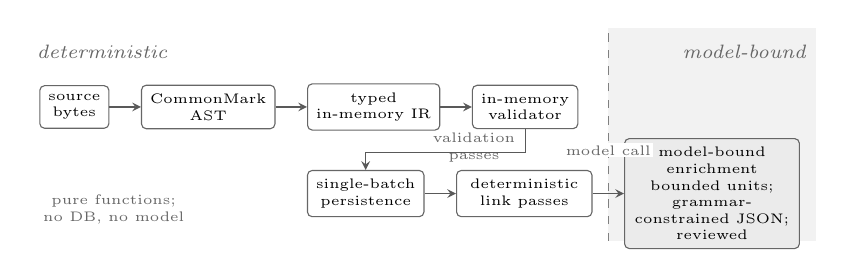
\begin{tikzpicture}[x=1mm,y=1mm,
    stg/.style={draw=black!60,rounded corners=0.6mm,fill=white,align=center,
                inner sep=1.1mm,font=\tiny},
    mdl/.style={stg,fill=black!8},
    rel/.style={-{stealth},line width=0.4pt,black!65},
    elab/.style={font=\tiny,text=black!60,align=center,inner sep=0.4mm},
    zone/.style={font=\scriptsize\itshape,text=black!60}]

\node[stg] (b) at (7,17) {source\\bytes};
\node[stg,right=4mm of b] (a) {CommonMark\\AST};
\node[stg,right=4mm of a] (i) {typed\\in-memory IR};
\node[stg,right=4mm of i] (v) {in-memory\\validator};
\node[stg] (p) at (44,6) {single-batch\\persistence};
\node[stg,text width=15mm,right=4mm of p] (l) {deterministic\\link passes};
\node[mdl,text width=20mm,right=4mm of l] (m) {model-bound\\enrichment\\bounded units;
    grammar-constrained JSON;\\reviewed};

\coordinate (boundary) at ($(l.east)!0.5!(m.west)$);
\coordinate (floor) at (0,0);
\coordinate (ceiling) at (0,27);
\coordinate (rightedge) at ([xshift=2mm]m.east);
\begin{scope}[on background layer]
\fill[black!5] (boundary |- floor) rectangle (rightedge |- ceiling);
\end{scope}
\draw[dashed,black!50,line width=0.4pt] (boundary |- floor) -- (boundary |- ceiling);
\node[zone,anchor=west] at (1,24) {deterministic};
\node[zone,anchor=east] at (rightedge |- 0,24) {model-bound};

\node[elab] at (12,4) {pure functions;\\no DB, no model};

\draw[rel] (b) -- (a);
\draw[rel] (a) -- (i);
\draw[rel] (i) -- (v);
\draw[rel] (v.south) -- ++(0,-3mm) -| (p.north);
\node[elab,anchor=east] at ([xshift=-0.8mm,yshift=-2.3mm]v.south) {validation\\passes};
\draw[rel] (p) -- (l);
\draw[rel] (l) -- (m);
\node[elab,fill=white,inner sep=0.3mm] at (boundary |- 0,11.5) {model call};
\end{tikzpicture}
\end{document}
